\chapter{Modulo configurazione prodotto}\label{chapter:Configurazione}
\section{Scopo del modulo}
Il vero salto di qualità, rispetto all'attuale metodo di creazione delle offerte,
è l'introduzione di un modulo di configurazione prodotto.
Come citato nell'introduzione~\ref{chapter:introduction}, l'azienda ha un modello di business
di tipo \ac{ETO}. Questo modello comporta la produzione di prodotti realizzati
su misura per il cliente, utilizzando però componenti standardizzati.
L'utilizzo di prodotti standardizzati permette di individuare e catalogare 
le possibili varianti di prodotto; tali varianti vengono utilizzate per creare
un sistema di configurazione che permetta di anticipare già in fase di vendita i prodotti necessari.
Il numero di tipologie di prodotto e di varianti per ciascuna tipologia è molto elevato,
e non è possibile conoscere a priori né le regole che governano la configurazione di un prodotto
 né i componenti che lo compongono.
Si è dovuto quindi cercare di realizzare una struttura ed un algoritmo che permettessero
di configurare un prodotto all'interno del sistema. L'utente deve
poter creare regole e combinarle in modo agile.
Oltre allo studio della configurazione stessa, è stato
necesario studiare un sistema che guidasse l'utente nella scelta del prodotto da configurare.
L'algoritmo implementato si suddivide in tre fasi principali:
\begin{itemize}
    \item \textbf{Fase di scelta del modello:} mediante alberi di scelta
    l'utente discende da concetti generali, come lo scopo del componente (es. "stoccaggio prodotti"),
     fino alla tipologia di prodotto(es: silo in acciaio), per arrivare al modello specifico
      da configurare(es: "forma quadrata").
     Questo modello ad albero guida l'utente.
    \item \textbf{Fase di configurazione:} in questa fase vengono proposti all'utente delle
    opzioni di scelta sottorma di dropdown  o testo libero.
    Ogni dropdown o casella appartiene ad una sola tipologia di proprietà utilizzata nelle regole del prodotto. 
    Il menù è generato dinamicamente filtratndo le proprietà  associate alle regole in base al macrogruppo scelto.
    \item \textbf{Fase di scelta dei componenti:} compilate 
    le scelte precedenti, i componenti del macrogruppo vengono sottoposti a filtro in base alle regole associate ad ognuno di essi.
    In questo modo vengono proposti all'utente solo i componenti che rispettano le regole, e quindi disponibili per la configurazione.
    I compoennti proposti a loro volta possono essere esclusi dall'utente.
    \item \textbf{Generazione codice:} questa fase 
    finale è la più delicata dell'implementazione dell'algoritmo, in quanto, in base ai codici scelti, si hanno
    due alternative:
    \begin{itemize}
        \item \textbf{Configurazione esistente:} si ricerca nel database se esiste già una configurazione
        di quel prodotto con i codici scelti.
         In caso positivo si propone all'utente di utilizzare quella configurazione.
        \item \textbf{Configurazione inesistente:} in caso negativo, 
        si genera un nuovo codice di configurazione per il prodotto, che viene salvato nel database.
    \end{itemize}
\end{itemize}
\subsection{Scelta macrogruppo da configurare}
La realizzazione dell'albero di scelta è stata fatta sfruttando
le tabelle già presenti nel database, in particolare le tabelle \textit{prodotto}, \textit{prodotti\_composizioni} e la tabella
di lookup \textit{tipi\_prodotto}.
Si sono generate tre nuove tipologie di prodotto, ovvero:
\begin{itemize}
  \item \textbf{Iniziale:} rappresenta il concetto generale del prodotto,
   e permette di guidare l'utente nella scelta del modello da configurare. Questo tipologia permette un punto di
  partenza per l'algoritmo di configurazione.
  \item \textbf{Mappa:} rappresenta un concetto intermedio, e permette di guidare l'utente nella scelta del modello da configurare.
  Questi prodotti sono stati inseriti all'interno delle distinte dei prodotti di tipo iniziale.
  A loro volta possono contenere prodotti di tipo mappa o macrogruppo, per continuare la discesa nell'albero di scelta.
  \item \textbf{Macrogruppo:} rappresenta il contenitore dei componenti del modello da configurare.
  Ad ogni prodotto del macrogruppo sono associate delle regole che ne determinano la disponibilità nella configurazione.
   Questi prodotti sono stati inseriti all'interno delle distinte dei prodotti di tipo mappa.
\end{itemize}
 Questa struttura permette la realizzazione di un albero ampiamente scalabile,
  in quanto è possibile aggiungere nuovi prodotti senza dover modificare l'algoritmo.
L'albero in questione è osservabile in figura~\ref{fig:Albero di scelta prodotto}.
\begin{figure}[H]
    \centering
    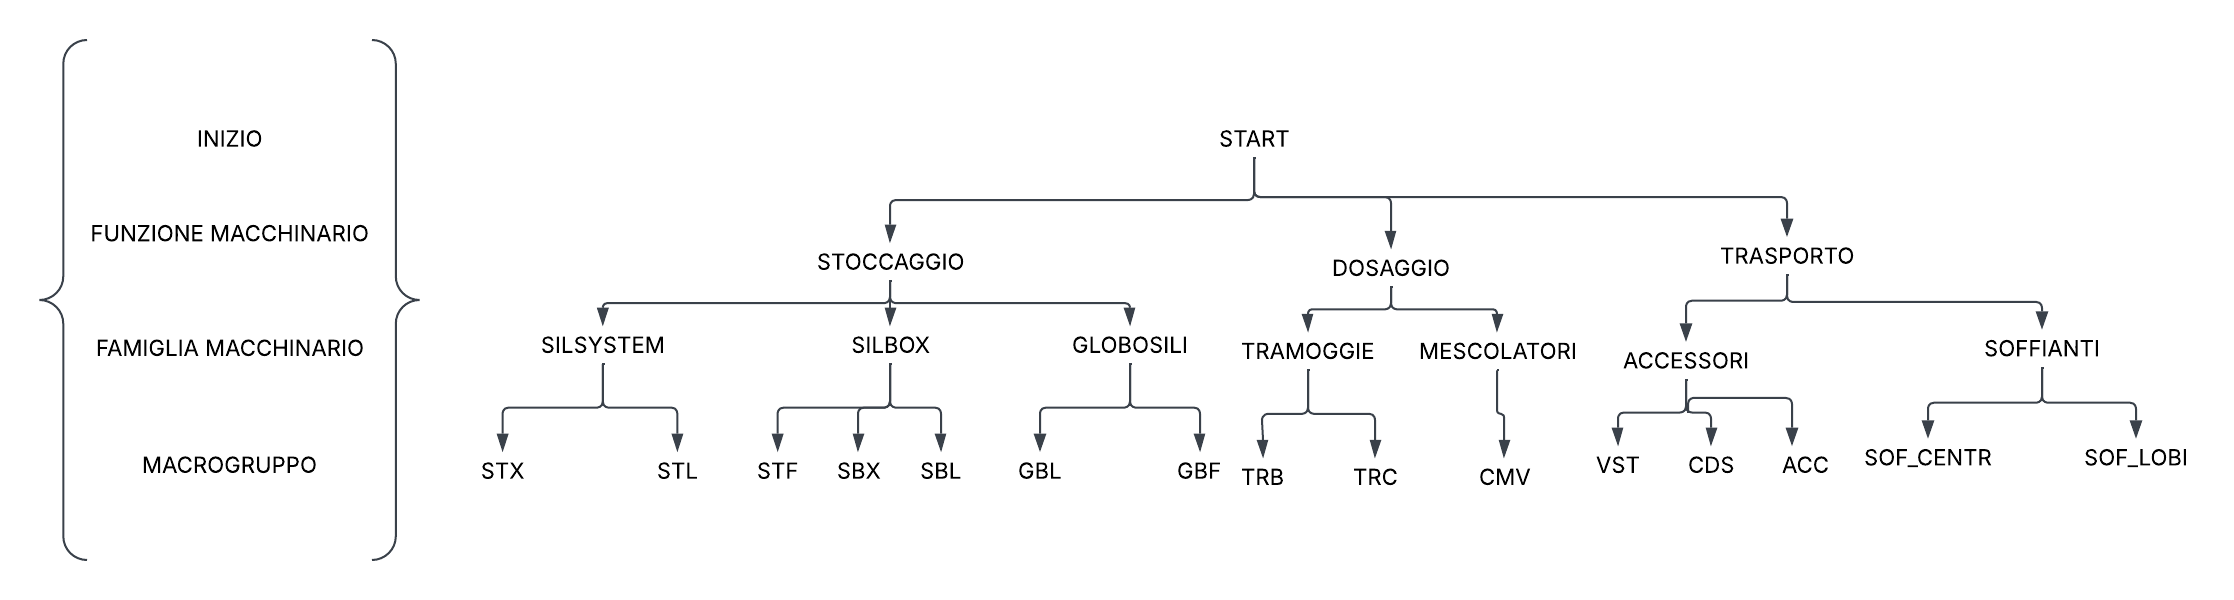
\includegraphics[width=1\linewidth]{figures/AlberoScelte.png}
    \caption{Albero di scelta prodotto}\label{fig:Albero di scelta prodotto}
\end{figure}
\subsection{Implementazione delle regole}
I macrogruppi contengono al loro interno tutti i componenti possibili per la configurazione del prodotto.
A ogni componente sono state associate n regole che, se valide, determinano la sua disponibilità nella configurazione.
A ogni regola, a sua volta, è associata una proprietà di riferimento, un operatore logico e un valore di riferimento.
Le proprietà possono essere create dall'utente configuratore,
e altre alla creazione di tali proprità l'utete può creare dei valori standard della stessa, che
verranno proposti all'utente finale se compare tale proprietà nella configurazione.
Gli operatori possono essere di tipo logico, come "uguale a", "maggiore di", "minore di" o di "LIKE".
Solo l'operatore uguale avrà un dropdown con i valori standard della proprietà, 
mentre gli altri operatori permetteranno all'utente di inserire un valore libero o scelta da quelli disponibili.
\subsection{Generazione dell'interfaccia utente}
L'interfaccia utente con le possibili domande di configurazione
viene generata filtrando dinamicamente tutte le proprietà di riferimento delle regole, in base al macrogruppo scelto.
Viene messo in join i componenti, le regole e le proprietà, e successivamente prese solo questultime tramite un \textit{DISTINCT},
 in modo da avere una lista di proprietà univocue.
Questa query consente di ottenere tutte le proprietà univocue senza dover conoscere a priori 
le regole che governano la configurazione del prodotto.
\subsection{Struttura del database}
La realizzazione lato database è stata possibile introducendo due
nuove tabelle, la tabella \text{regole} e una di lookup \textit{operatorri\_logici}.
La struttura dinamica del database, implementata nelle prime fasi,
 ha permesso di realizzare l'implementazione in modo agile.
Di seguito, nella figura~\ref{fig:ER configuratore}, è possibile osservare il modello \ac{ER}
 del modulo di configurazione prodotto.
\begin{figure}[H]
    \centering
    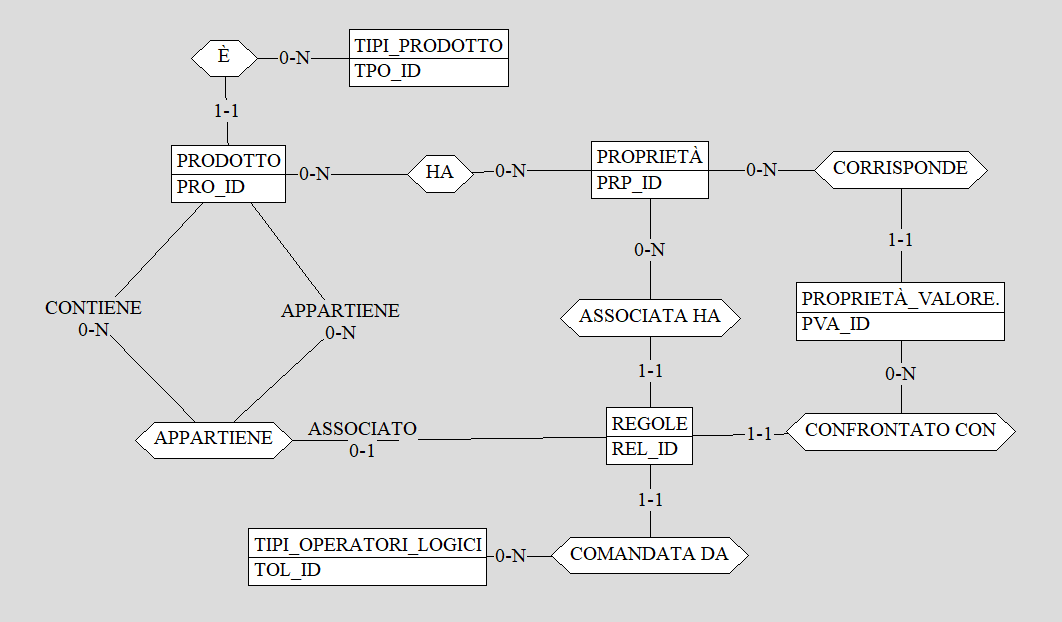
\includegraphics[width=0.9\linewidth]{figures/ER_Configuratore.png}
    \caption{Modello ER configuratore}\label{fig:ER configuratore}
\end{figure}
\subsection{Gestione del listino della configurazione}
Determinare il prezzo di una configurazione dinamica è un aspetto non banale,
 in quanto esso può dipendere o dai componenti scelti o da valori minimi di listino.
 Si è deciso per risolvere il problema di introdurre all'interno del macrogruppo dei 
 prodotti di tipologia \textit{listino}, che contengono le informazioni di prezzo minime per la configurazione.
 Ogni prodotto listino è soggetto come gli altri componenti alle regole del macrogruppo,
  e quindi può essere reso disponibile o meno in base alle scelte effettuate.
  Questo apporccio rende possibile determinare se il prezzo della somma dei componenti scelti è inferiore al prezzo minimo di listino,
   e in tal caso proporre all'utente il prezzo minimo.
I componenti di tipo listino saranno invisibili all'utente finale,
 in quanto non sono parte della configurazione, ma servono solo per determinare il prezzo minimo.
\section{Interfaccia grafica lato utente ed amministratore}
Le interfacce lato utente e amministratore sono profondamente diverse, in quanto, per offrire
all'utente un'esperienza di configurazione semplice e guidata,
la complessità è stata spostata lato amministratore.
\subsection{Lato utente}
L'esperienza di configurazione lato utente è stata realizzata dopo
un focus group con alcuni utenti, in cui si è cercato di capire quale potesse essere
il flusso di lavoro più semplice e intuitivo.
Si è deciso di proporre le scelte successive solo dopo aver effettuato la scelta precedente,
 in modo da guidare l'utente.
 Si è partiti dai concetti generali, come lo scopo del prodotto, fino ad arrivare al modello specifico da configurare.
 Nella figura~\ref{fig:Interfaccia lato utente} è possibile osservare l'interfaccia grafica lato utente.
 \begin{figure}[H]
    \centering
    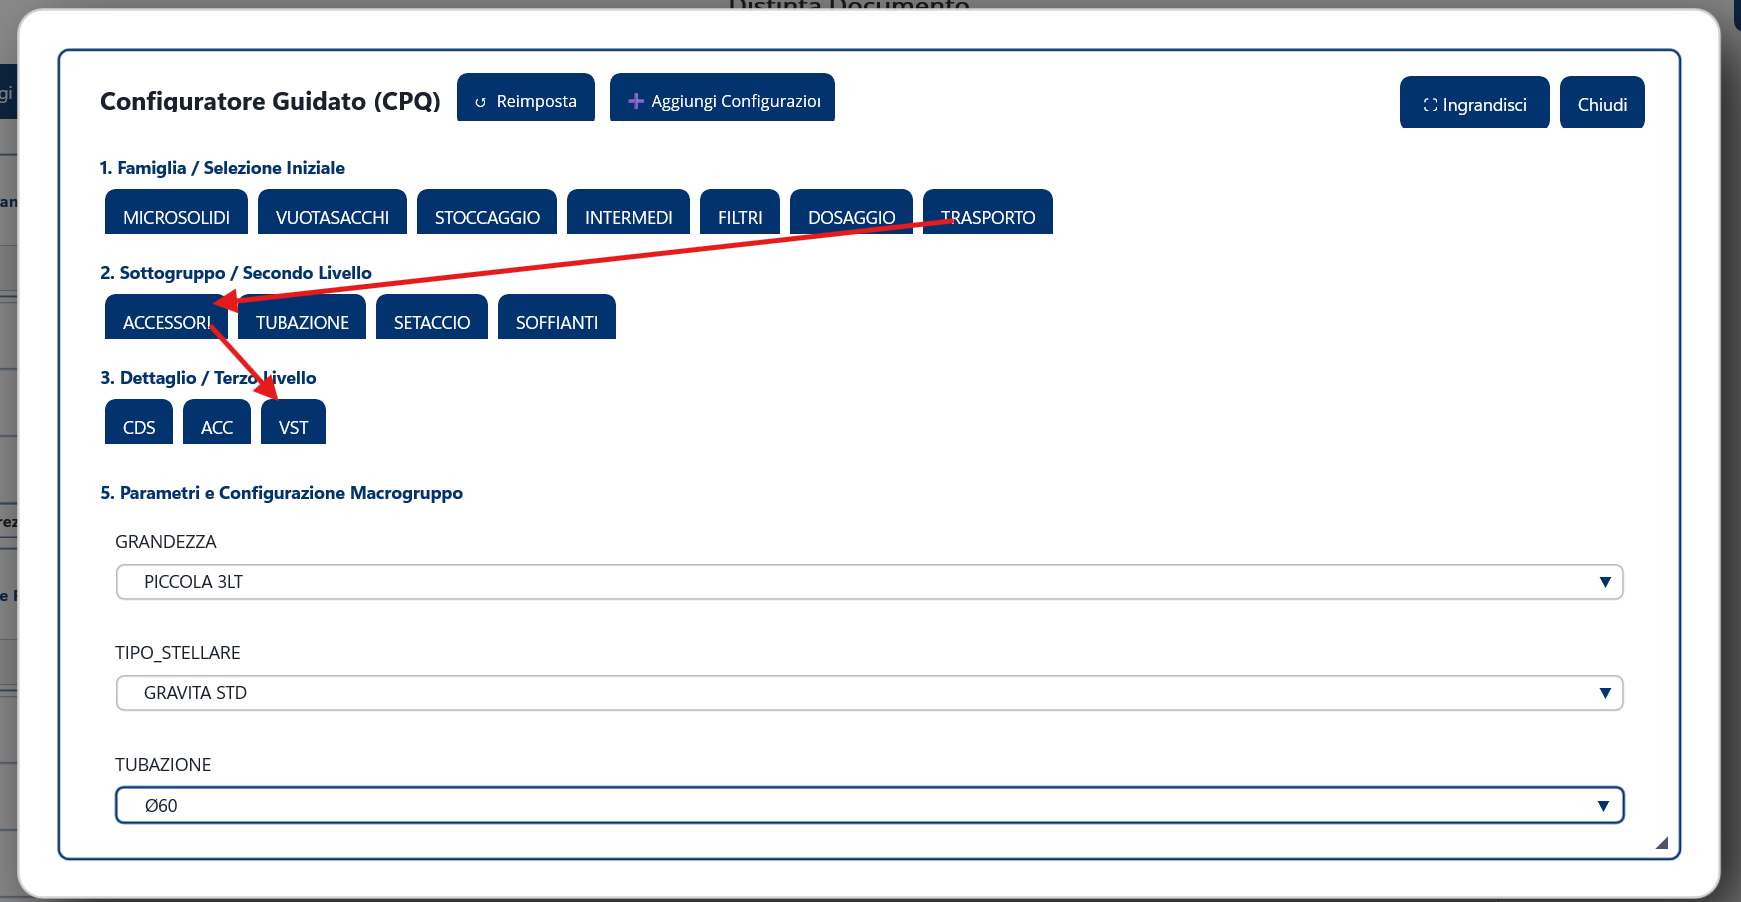
\includegraphics[width=0.9\linewidth]{figures/ConfigurazioneLatoUtente.png}
    \caption{Configurazione lato utente}\label{fig:Configurazione lato utente}
 \end{figure}
 Il risultato finale è visibile nella figura~\ref{fig:Risultato configurazione lato utente} sottostante.
  \begin{figure}[H]
    \centering
    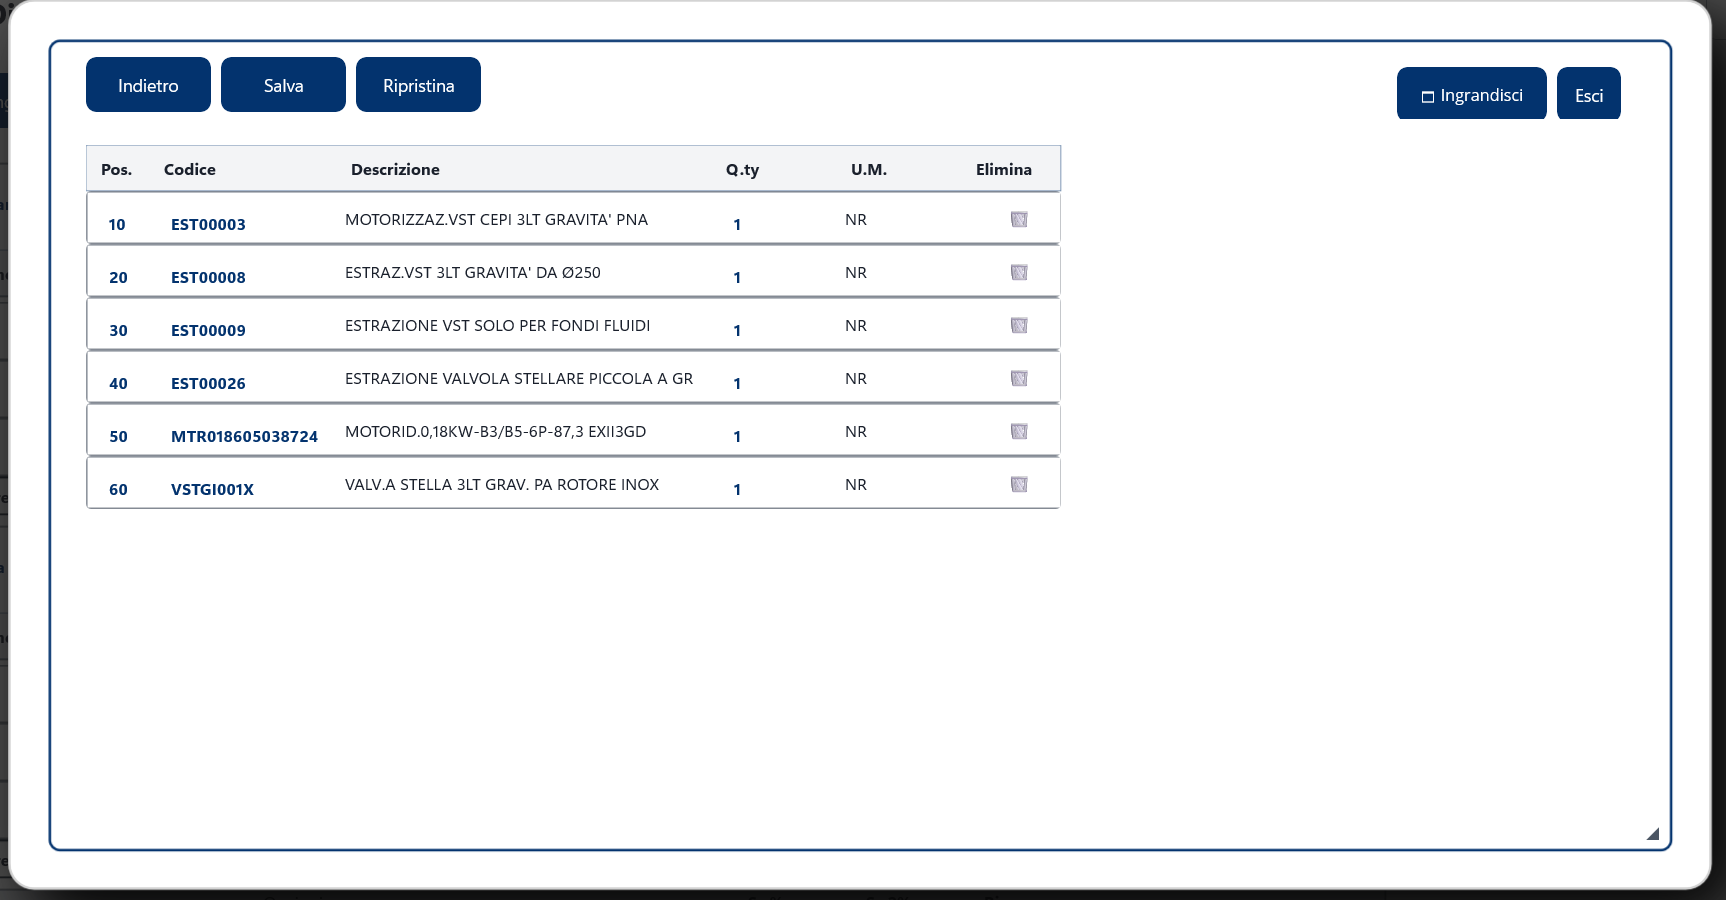
\includegraphics[width=0.9\linewidth]{figures/RisultatoConfigurazione.png}
    \caption{Risultato configurazione lato utente}\label{fig:Risultato configurazione lato utente}
 \end{figure}
 Al termine il codice generato o raccolto dal database viene aggiunto ai prodotti dell'offerta,
  e l'utente può proseguire con la creazione dell'offerta.
\subsection{Lato amministratore}
La creazione delle configurazioni passa dalla composizione dei macrogruppi.
Dopo aver compilato i componenti, a ognuno di essi possono essere assegnate una o più
regole.
L'assegnazione avviene aggiungendo la proprietà di riferimento, l'operatore logico e il valore che deve
 essere rispettato per rendere disponibile il componente.
 Di seguito l'interfaccia di aggiunta delle regole ad un componente,
  visibile in figura~\ref{fig:Interfaccia lato amministratore}.
  Si può notare a destra la scelta delle proprietà mediante filtri e a sinistra la lista delle
  regole già assegnate al componente.
  \begin{figure}[H]
    \centering
    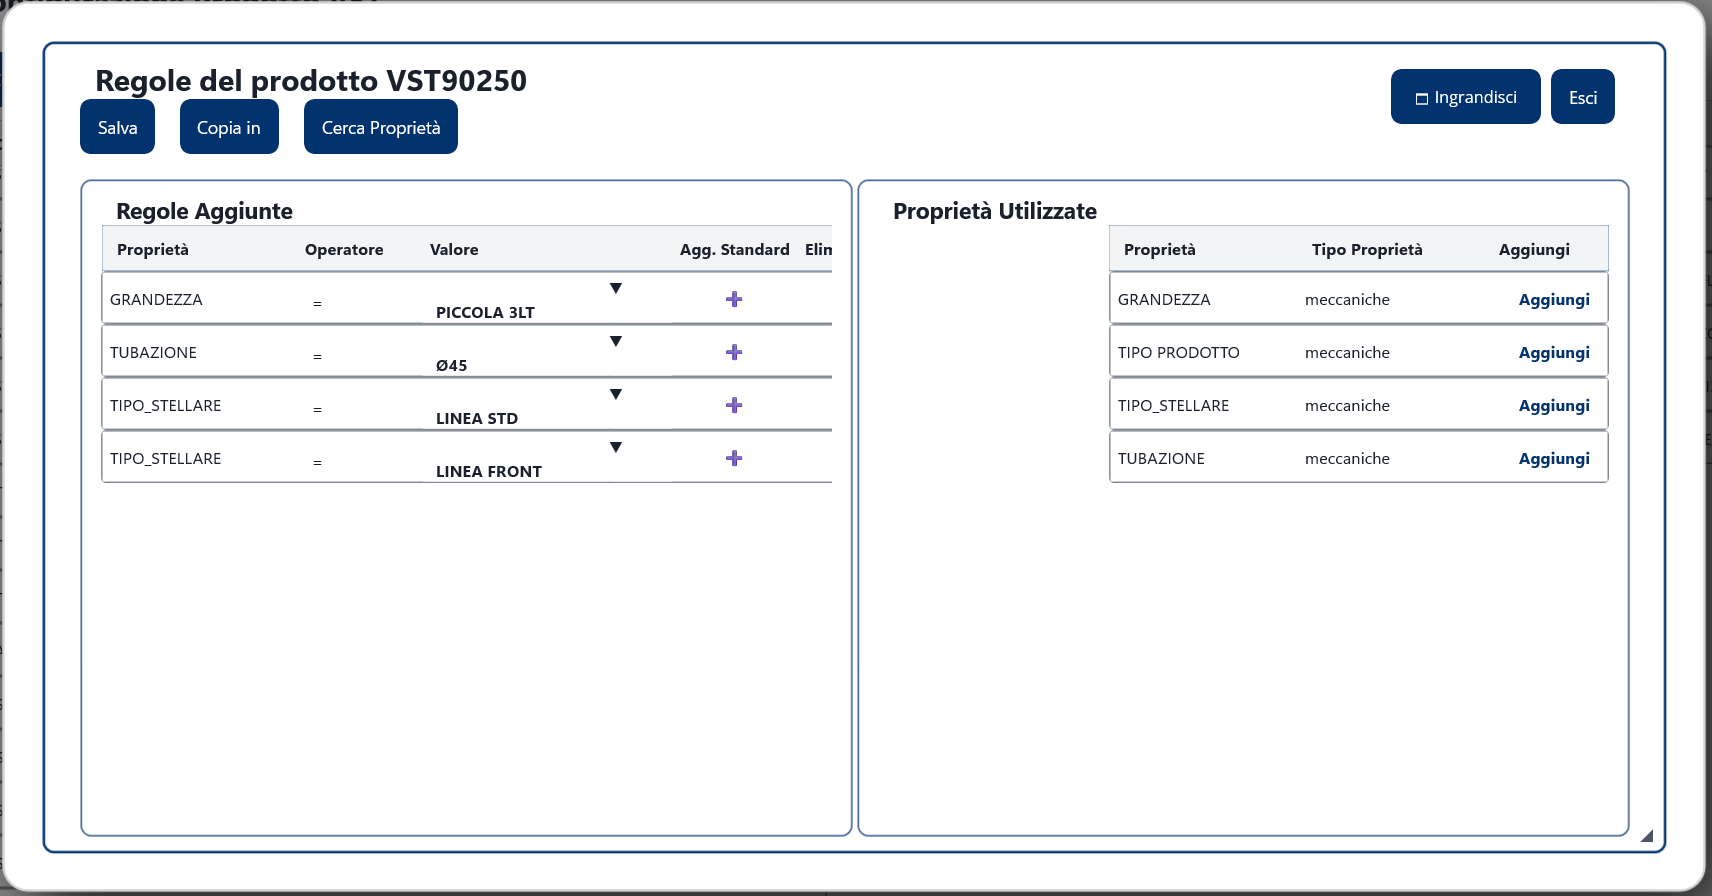
\includegraphics[width=0.9\linewidth]{figures/AggiuntaRegole.png}
    \caption{Aggiunta regole}\label{fig:Aggiunta regole lato amministratore}
  \end{figure}
  Dal focus group con gli utenti che potrebbero gestire la creazione è emerso che
  testare le regole è un aspetto fondamentale, in quanto permette di capire se le regole inserite
  sono corrette e se il flusso di configurazione è coerente.
  Si è quindi creata un'interfaccia di test delle regole, visibile in figura~\ref{fig:Test regole lato amministratore}.
  \begin{figure}[H]
    \centering
    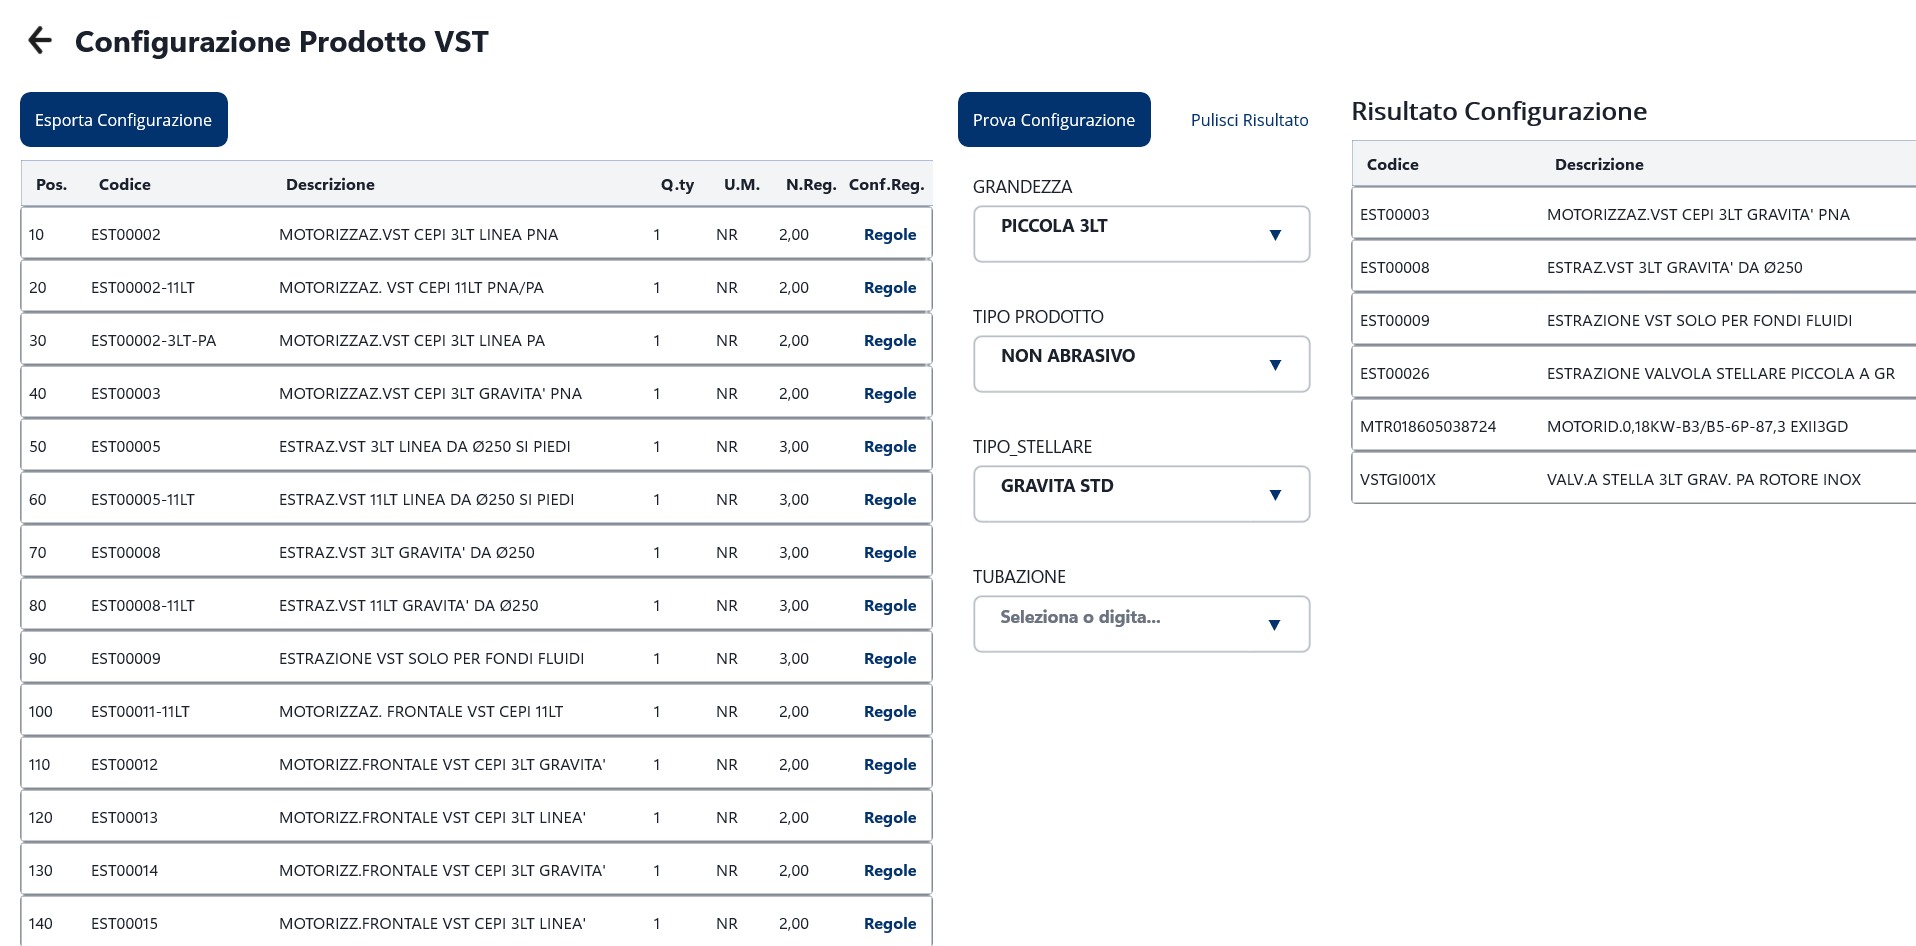
\includegraphics[width=0.9\linewidth]{figures/TestConfigurazione.png}
    \caption{Test regole lato amministratore}\label{fig:Test regole lato amministratore}
    \end{figure}